\documentclass[conference]{IEEEtran}
\IEEEoverridecommandlockouts
\usepackage{cite}
\usepackage{amsmath,amssymb,amsfonts}
\usepackage{graphicx}
\usepackage{textcomp}
\usepackage{xcolor}
\usepackage{booktabs}
\usepackage{array}
\usepackage{multirow}
\usepackage{url}
\usepackage[hidelinks]{hyperref}

\begin{document}

\title{NGO-Connect: An IEEE-Style Full-Stack Platform Study for Trustworthy Digital Philanthropy}

\author{
\IEEEauthorblockN{Utsav Anand, Thanvik S, Gujju Sunita, Yogesh, Deepu Mathew}
\IEEEauthorblockA{
Department of Computer Science and Engineering, CMR University, Bengaluru, India \\
utsav.anand@cmr.edu.in}
}

\maketitle

\begin{abstract}
Non-profit ecosystems often run on fragmented tooling for donations, volunteering, donor communication, and compliance. This paper presents an updated implementation study of NGO-Connect, a production-style web platform that unifies donors, NGOs, and administrators in one architecture. The current system integrates React 18 clients, an Express API, PostgreSQL with relational plus JSONB persistence, payment-gateway abstraction, webhooks with dead-letter replay, AI-assisted recommendations, and an Innovation Center for community giving circles, in-kind wishlists, emergency response, volunteer operations, CRM segmentation, and gamification. Static code analysis and platform instrumentation report 149 backend endpoints across 31 frontend routes, backed by 35 relational tables. End-to-end smoke execution over 35 scenario steps shows 21.69 ms mean latency per validated step (72 ms p90, 125 ms max). These results indicate that the platform can maintain operational reliability while expanding feature breadth and governance controls.
\end{abstract}

\begin{IEEEkeywords}
non-profit technology, full-stack engineering, PostgreSQL JSONB, payment gateway, webhooks, AI recommendation, innovation center, role-based access control
\end{IEEEkeywords}

\section{Introduction}
Digital philanthropy depends on trust, transparency, and low-friction participation. In practice, many NGOs rely on disconnected tools for fundraising, beneficiary reporting, volunteer coordination, and stakeholder communication, resulting in data silos and operational delay. NGO-Connect was built as an integrated platform to close these gaps through a role-aware workflow for \textit{users} (donors/volunteers), \textit{NGOs}, and \textit{administrators}.

The project has evolved from a campaign/donation MVP into a broader operations stack with webhook reliability, innovation workflows, and AI-assisted services. This updated paper documents the complete implemented surface and its engineering characteristics.

\subsection{Contributions}
The paper makes four concrete contributions:
\begin{enumerate}
  \item A complete, implementation-grounded architecture for NGO operations spanning fundraising, volunteering, CRM, moderation, and transparency.
  \item A gateway-first payment model with explicit confirmation, followed by domain recording (including Innovation Center giving circles).
  \item Reliability controls for outbound events via webhook logs, dead-letter handling, replay, metrics, export, and cleanup APIs.
  \item A feature-expansion analysis with measured endpoint, schema, and smoke-test performance metrics.
\end{enumerate}

\section{Related Work}
Prior studies emphasize the importance of digital trust for donation behavior and social engagement workflows. Modern web architecture guidance highlights layered API design and role-based authorization as essential for secure, multi-actor systems. Recent research on Retrieval-Augmented Generation (RAG) and recommendation ranking quality informs AI features in NGO-Connect, while operations guidance on tail latency and API security informs reliability hardening \cite{reactdocs,expressdocs,postgresdocs,jwt,rfc_tail,rag,owaspapi}.

\section{System Architecture}
\subsection{Stack and Layering}
NGO-Connect follows a three-tier model:
\begin{itemize}
  \item \textbf{Presentation tier:} React 18, route guards, role-specific dashboards, and innovation workspace.
  \item \textbf{Application tier:} Express route groups, JWT middleware, domain services, webhook workers, and AI utilities.
  \item \textbf{Data \& integration tier:} PostgreSQL relational tables with JSONB source documents, payment provider integration, and notification/webhook channels.
\end{itemize}

\begin{figure}[htbp]
\centerline{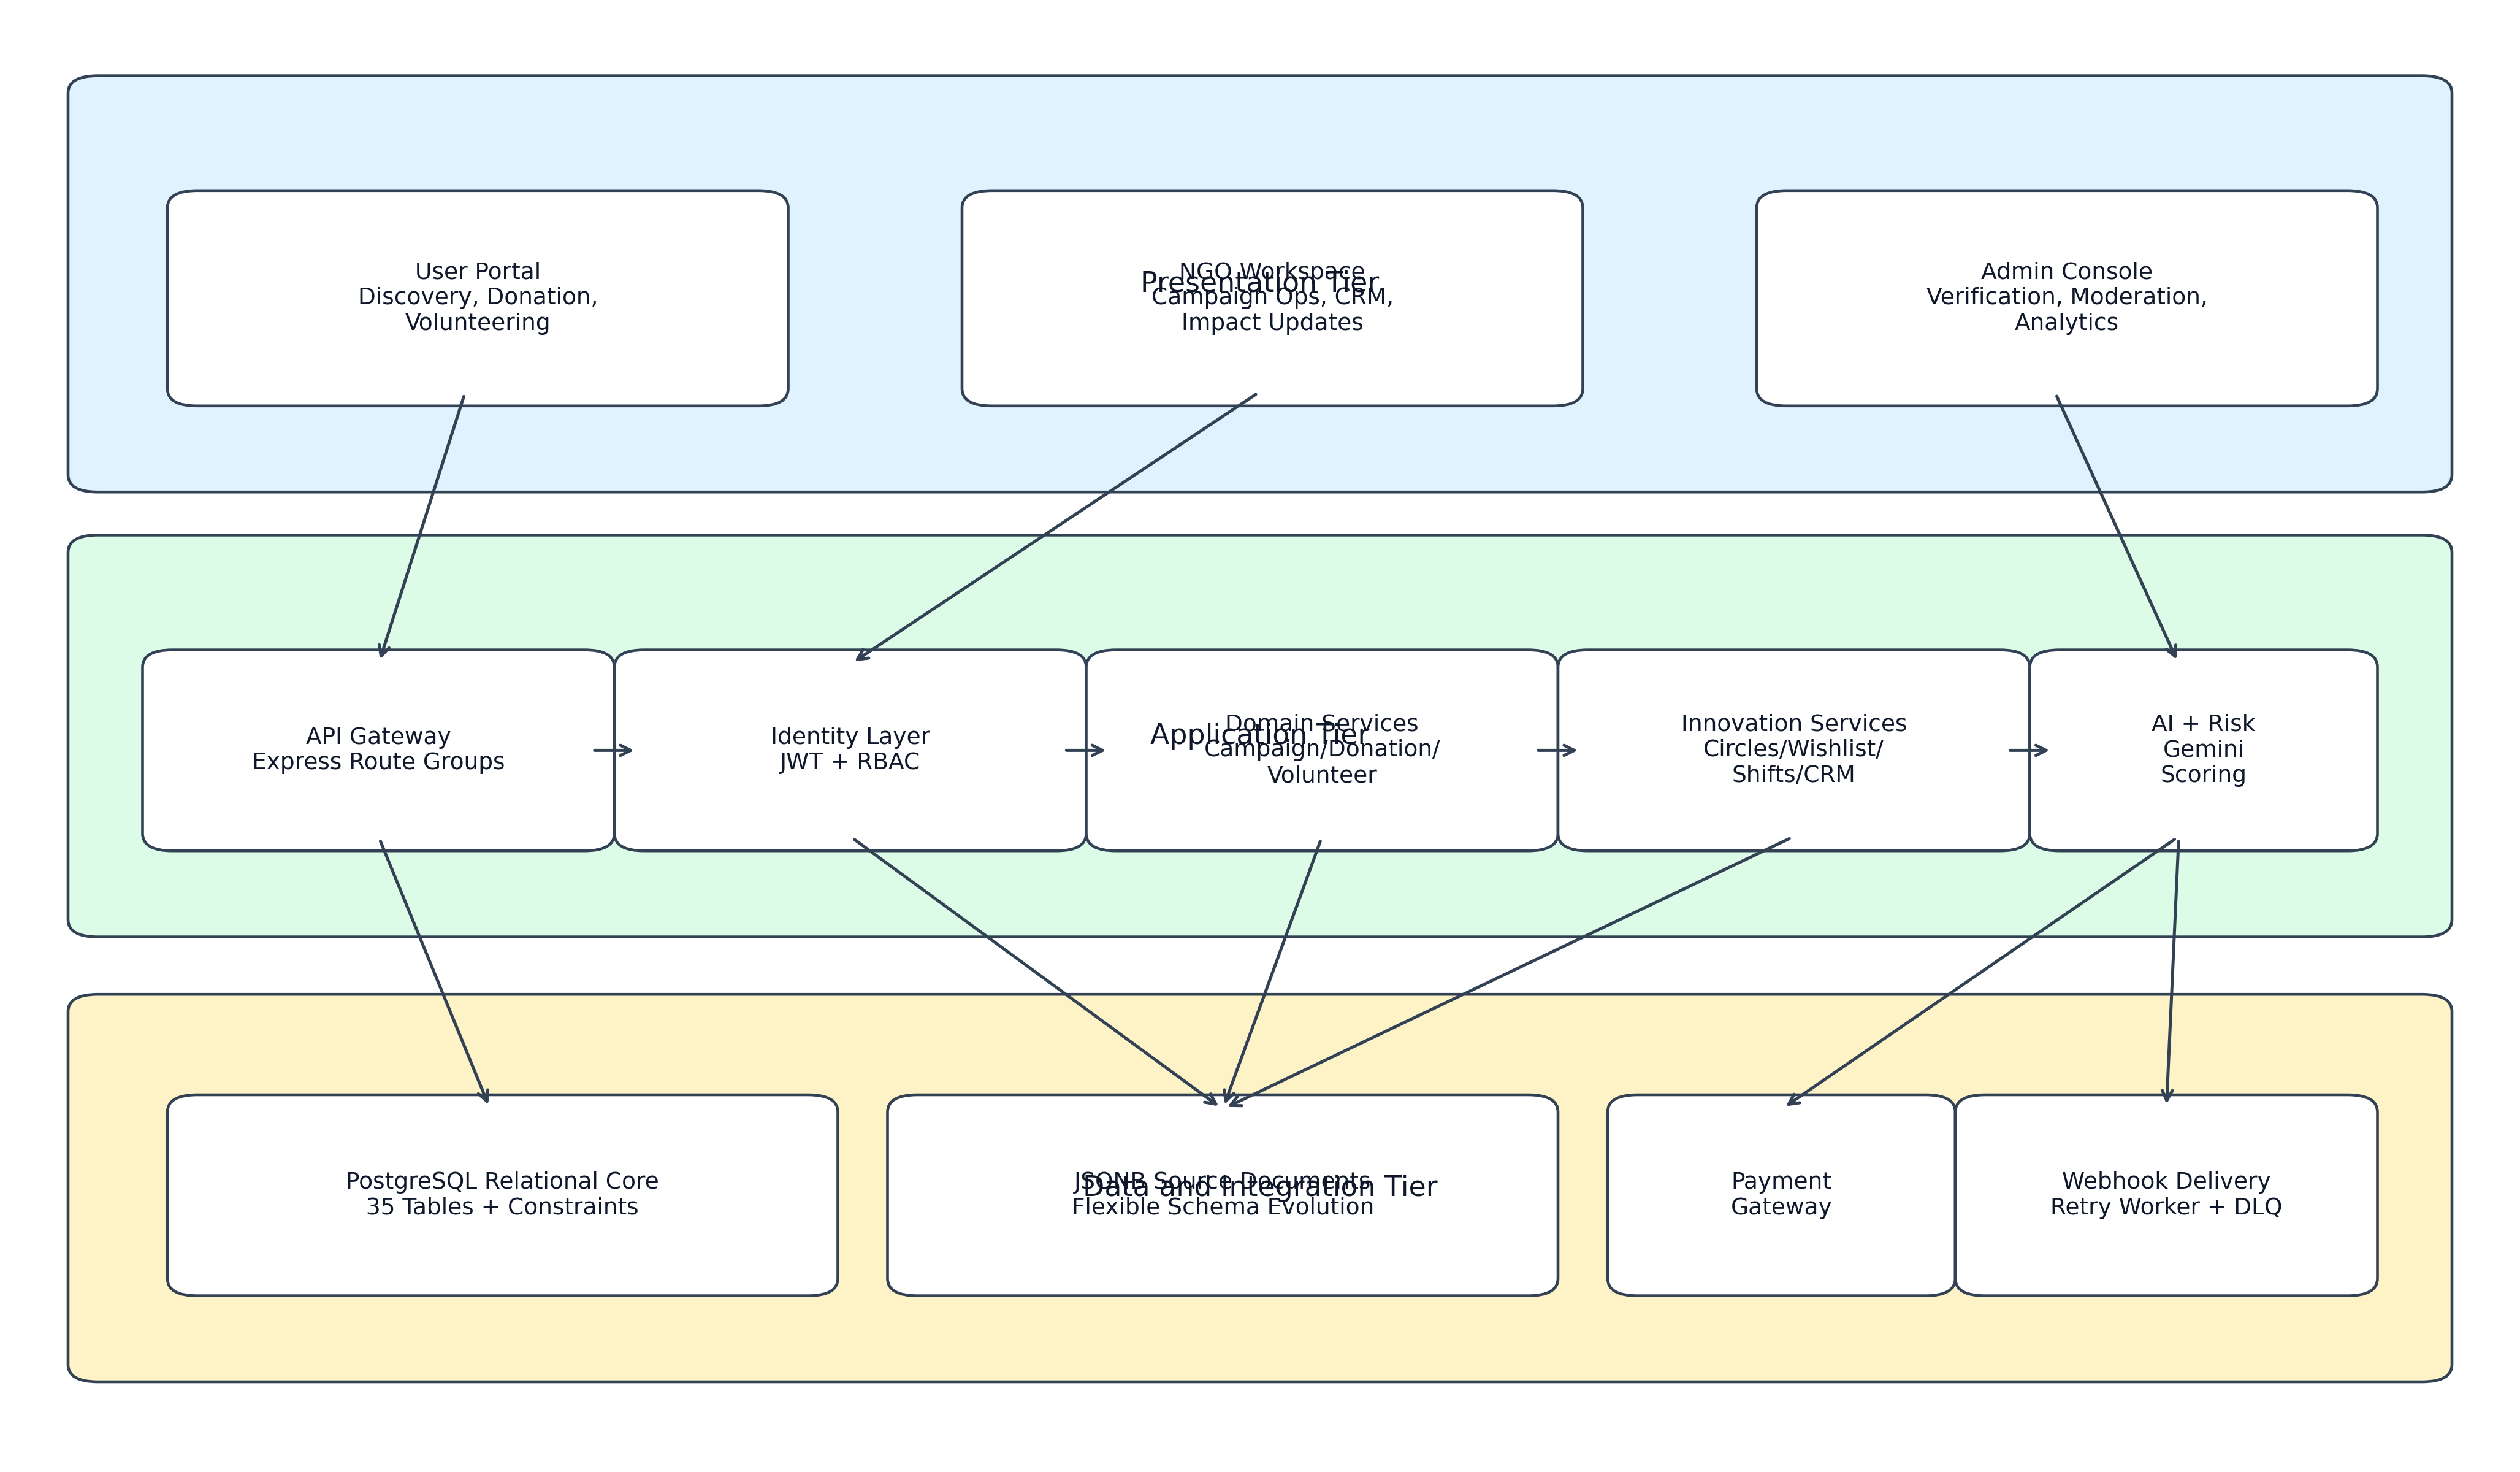
\includegraphics[width=\linewidth]{figures/system_architecture.png}}
\caption{Updated multi-tier NGO-Connect architecture with innovation and reliability services.}
\label{fig:arch}
\end{figure}

\subsection{Scale Snapshot from Source Analysis}
\begin{table}[htbp]
\caption{Platform Scale Snapshot}
\begin{center}
\begin{tabular}{|l|c|}
\hline
\textbf{Metric} & \textbf{Value} \\
\hline
Backend route endpoints & 149 \\
\hline
Frontend route paths & 31 \\
\hline
Relational tables & 35 \\
\hline
Innovation route endpoints & 44 \\
\hline
Admin route endpoints & 25 \\
\hline
\end{tabular}
\label{tab:snapshot}
\end{center}
\end{table}

\begin{figure}[htbp]
\centerline{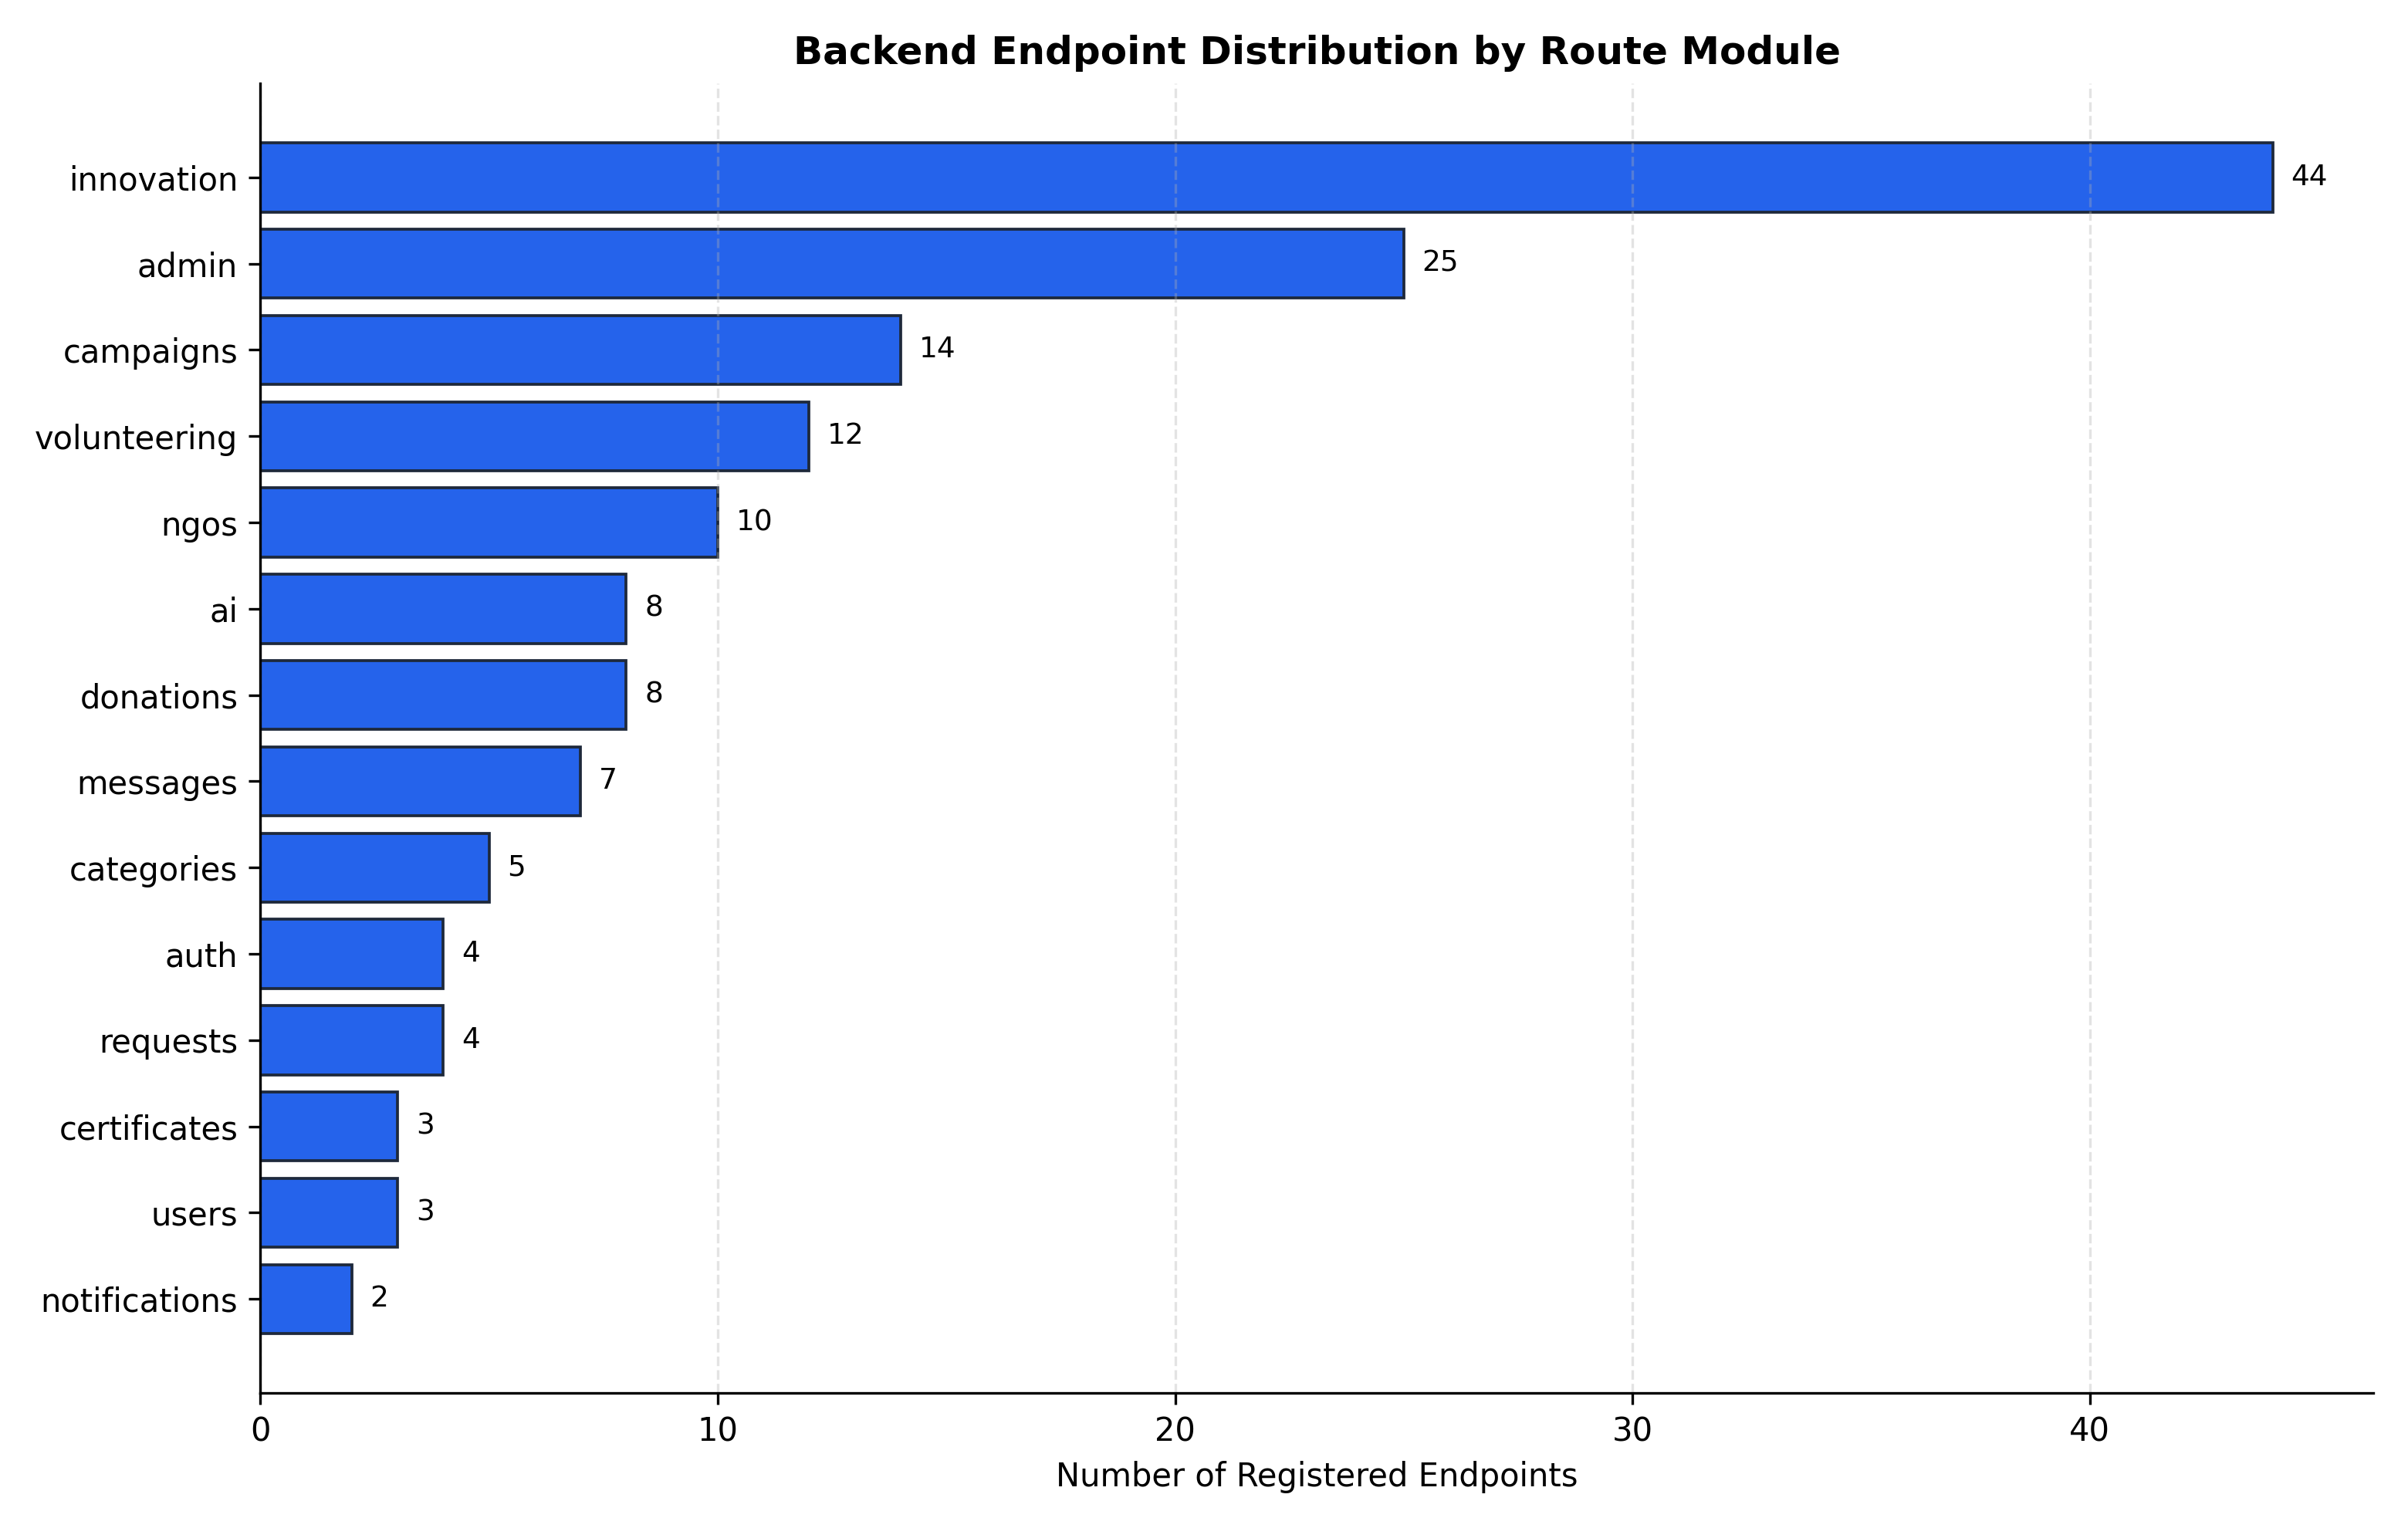
\includegraphics[width=\linewidth]{figures/endpoint_distribution.png}}
\caption{Endpoint distribution by backend module.}
\label{fig:endpoints}
\end{figure}

\begin{table}[htbp]
\caption{Top Route Modules by Endpoint Mix}
\begin{center}
\begin{tabular}{|l|c|c|c|c|c|}
\hline
\textbf{Module} & \textbf{Total} & \textbf{GET} & \textbf{POST} & \textbf{PUT} & \textbf{DELETE} \\
\hline
innovation & 44 & 20 & 24 & 0 & 0 \\
admin & 25 & 14 & 6 & 4 & 1 \\
campaigns & 14 & 8 & 6 & 0 & 0 \\
volunteering & 12 & 6 & 4 & 0 & 2 \\
ngos & 10 & 5 & 4 & 1 & 0 \\
ai & 8 & 1 & 7 & 0 & 0 \\
donations & 8 & 4 & 4 & 0 & 0 \\
messages & 7 & 3 & 4 & 0 & 0 \\
categories & 5 & 2 & 1 & 1 & 1 \\
auth & 4 & 1 & 2 & 1 & 0 \\
\hline
\end{tabular}
\label{tab:modules}
\end{center}
\end{table}

\begin{table}[htbp]
\caption{HTTP Method Distribution}
\begin{center}
\begin{tabular}{|l|c|}
\hline
\textbf{Method} & \textbf{Count} \\
\hline
GET & 72 \\
POST & 64 \\
PUT & 9 \\
DELETE & 4 \\
PATCH & 0 \\
\hline
\end{tabular}
\label{tab:methods}
\end{center}
\end{table}

\section{Complete Feature Coverage}
\subsection{Core Product Modules}
The implemented system includes:
\begin{itemize}
  \item Authentication, profile management, and role-based route protection.
  \item Campaign publication and detail updates with engagement tracking.
  \item Donation initiation/confirmation pipeline with receipts and certificate approval flow.
  \item Volunteer opportunity lifecycle and campaign-volunteering lifecycle.
  \item NGO dashboard team documentation with members list, role distribution, task contributions, and badge metadata.
  \item User-NGO messaging threads and help/support requests.
  \item Admin verification, moderation, notifications, request management, analytics, and user management.
  \item AI endpoints for recommendations, proposal draft generation, and campaign forecast assistance.
\end{itemize}

\subsection{Innovation Center Modules}
The Innovation Center expands operations with giving circles, in-kind wishlists, emergency feed contributions, shift management, donor CRM segmentation, corporate matching, impact updates, volunteer endorsements, and gamification leaderboard views.

\begin{figure}[htbp]
\centerline{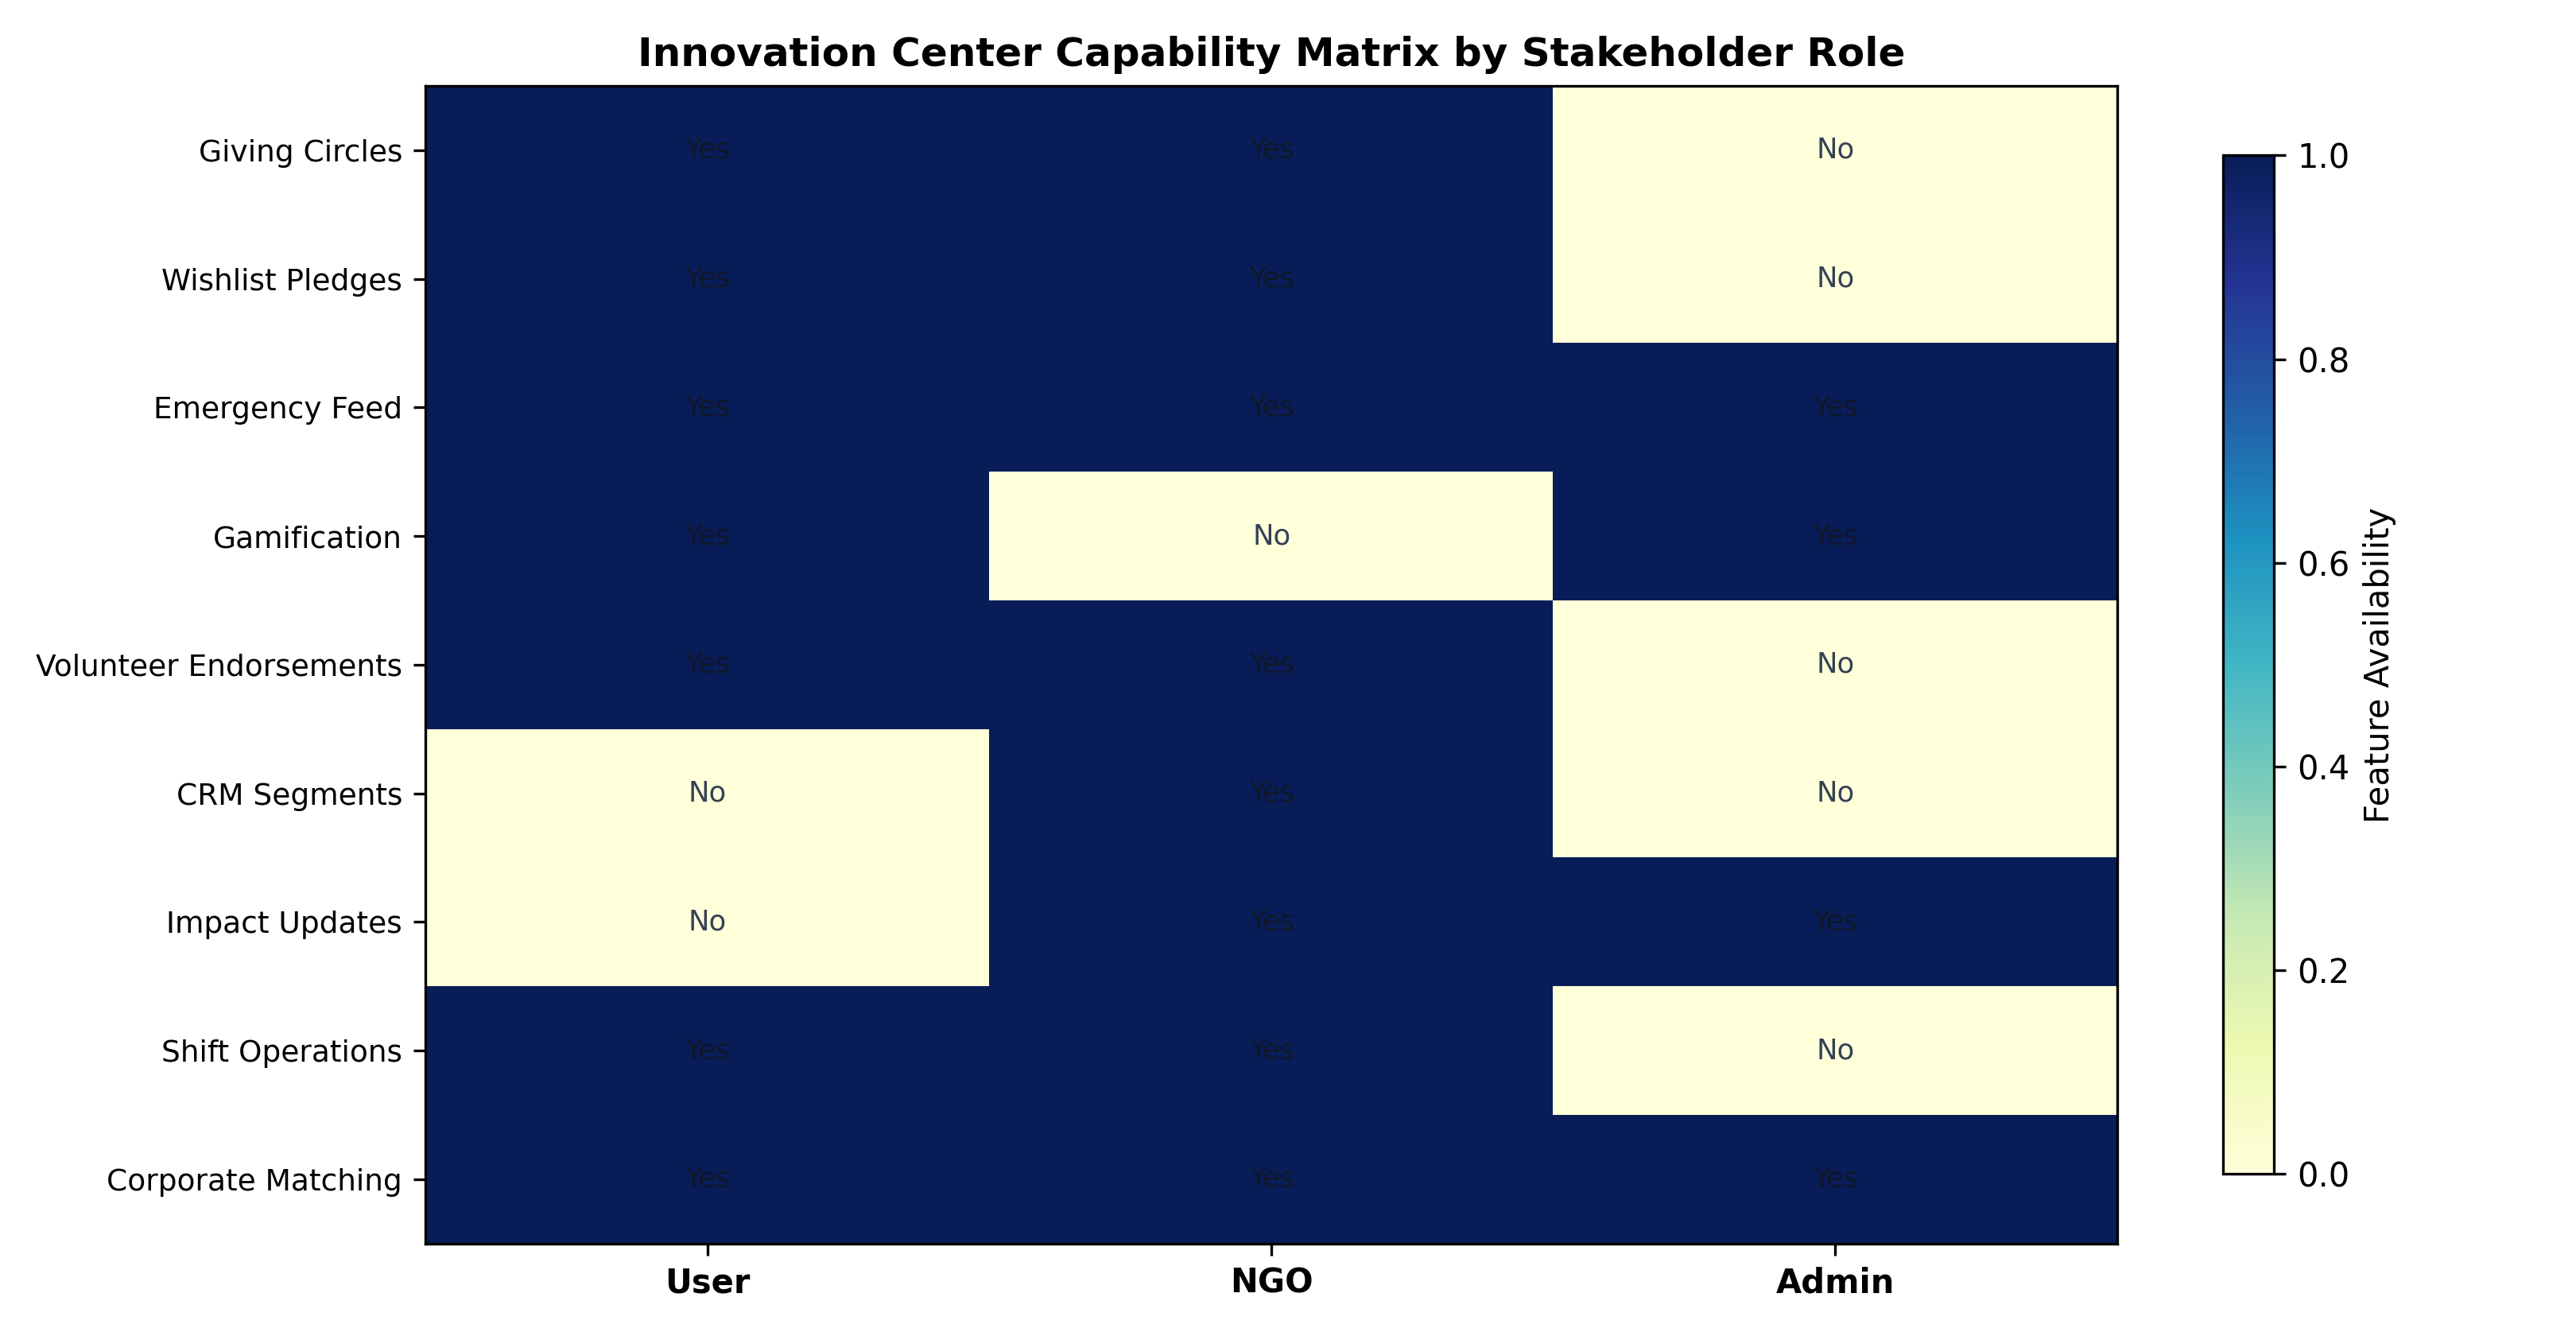
\includegraphics[width=\linewidth]{figures/innovation_feature_matrix.png}}
\caption{Innovation capability matrix across user, NGO, and admin stakeholders.}
\label{fig:innovationmatrix}
\end{figure}

\subsection{Payment and Trust Workflow}
The monetary flow is gateway-first. A contribution is initiated, the provider checkout completes, and only then is final state recorded in the domain module. This now applies to emergency campaign contributions and giving-circle contributions in the innovation workflow.

\begin{figure}[htbp]
\centerline{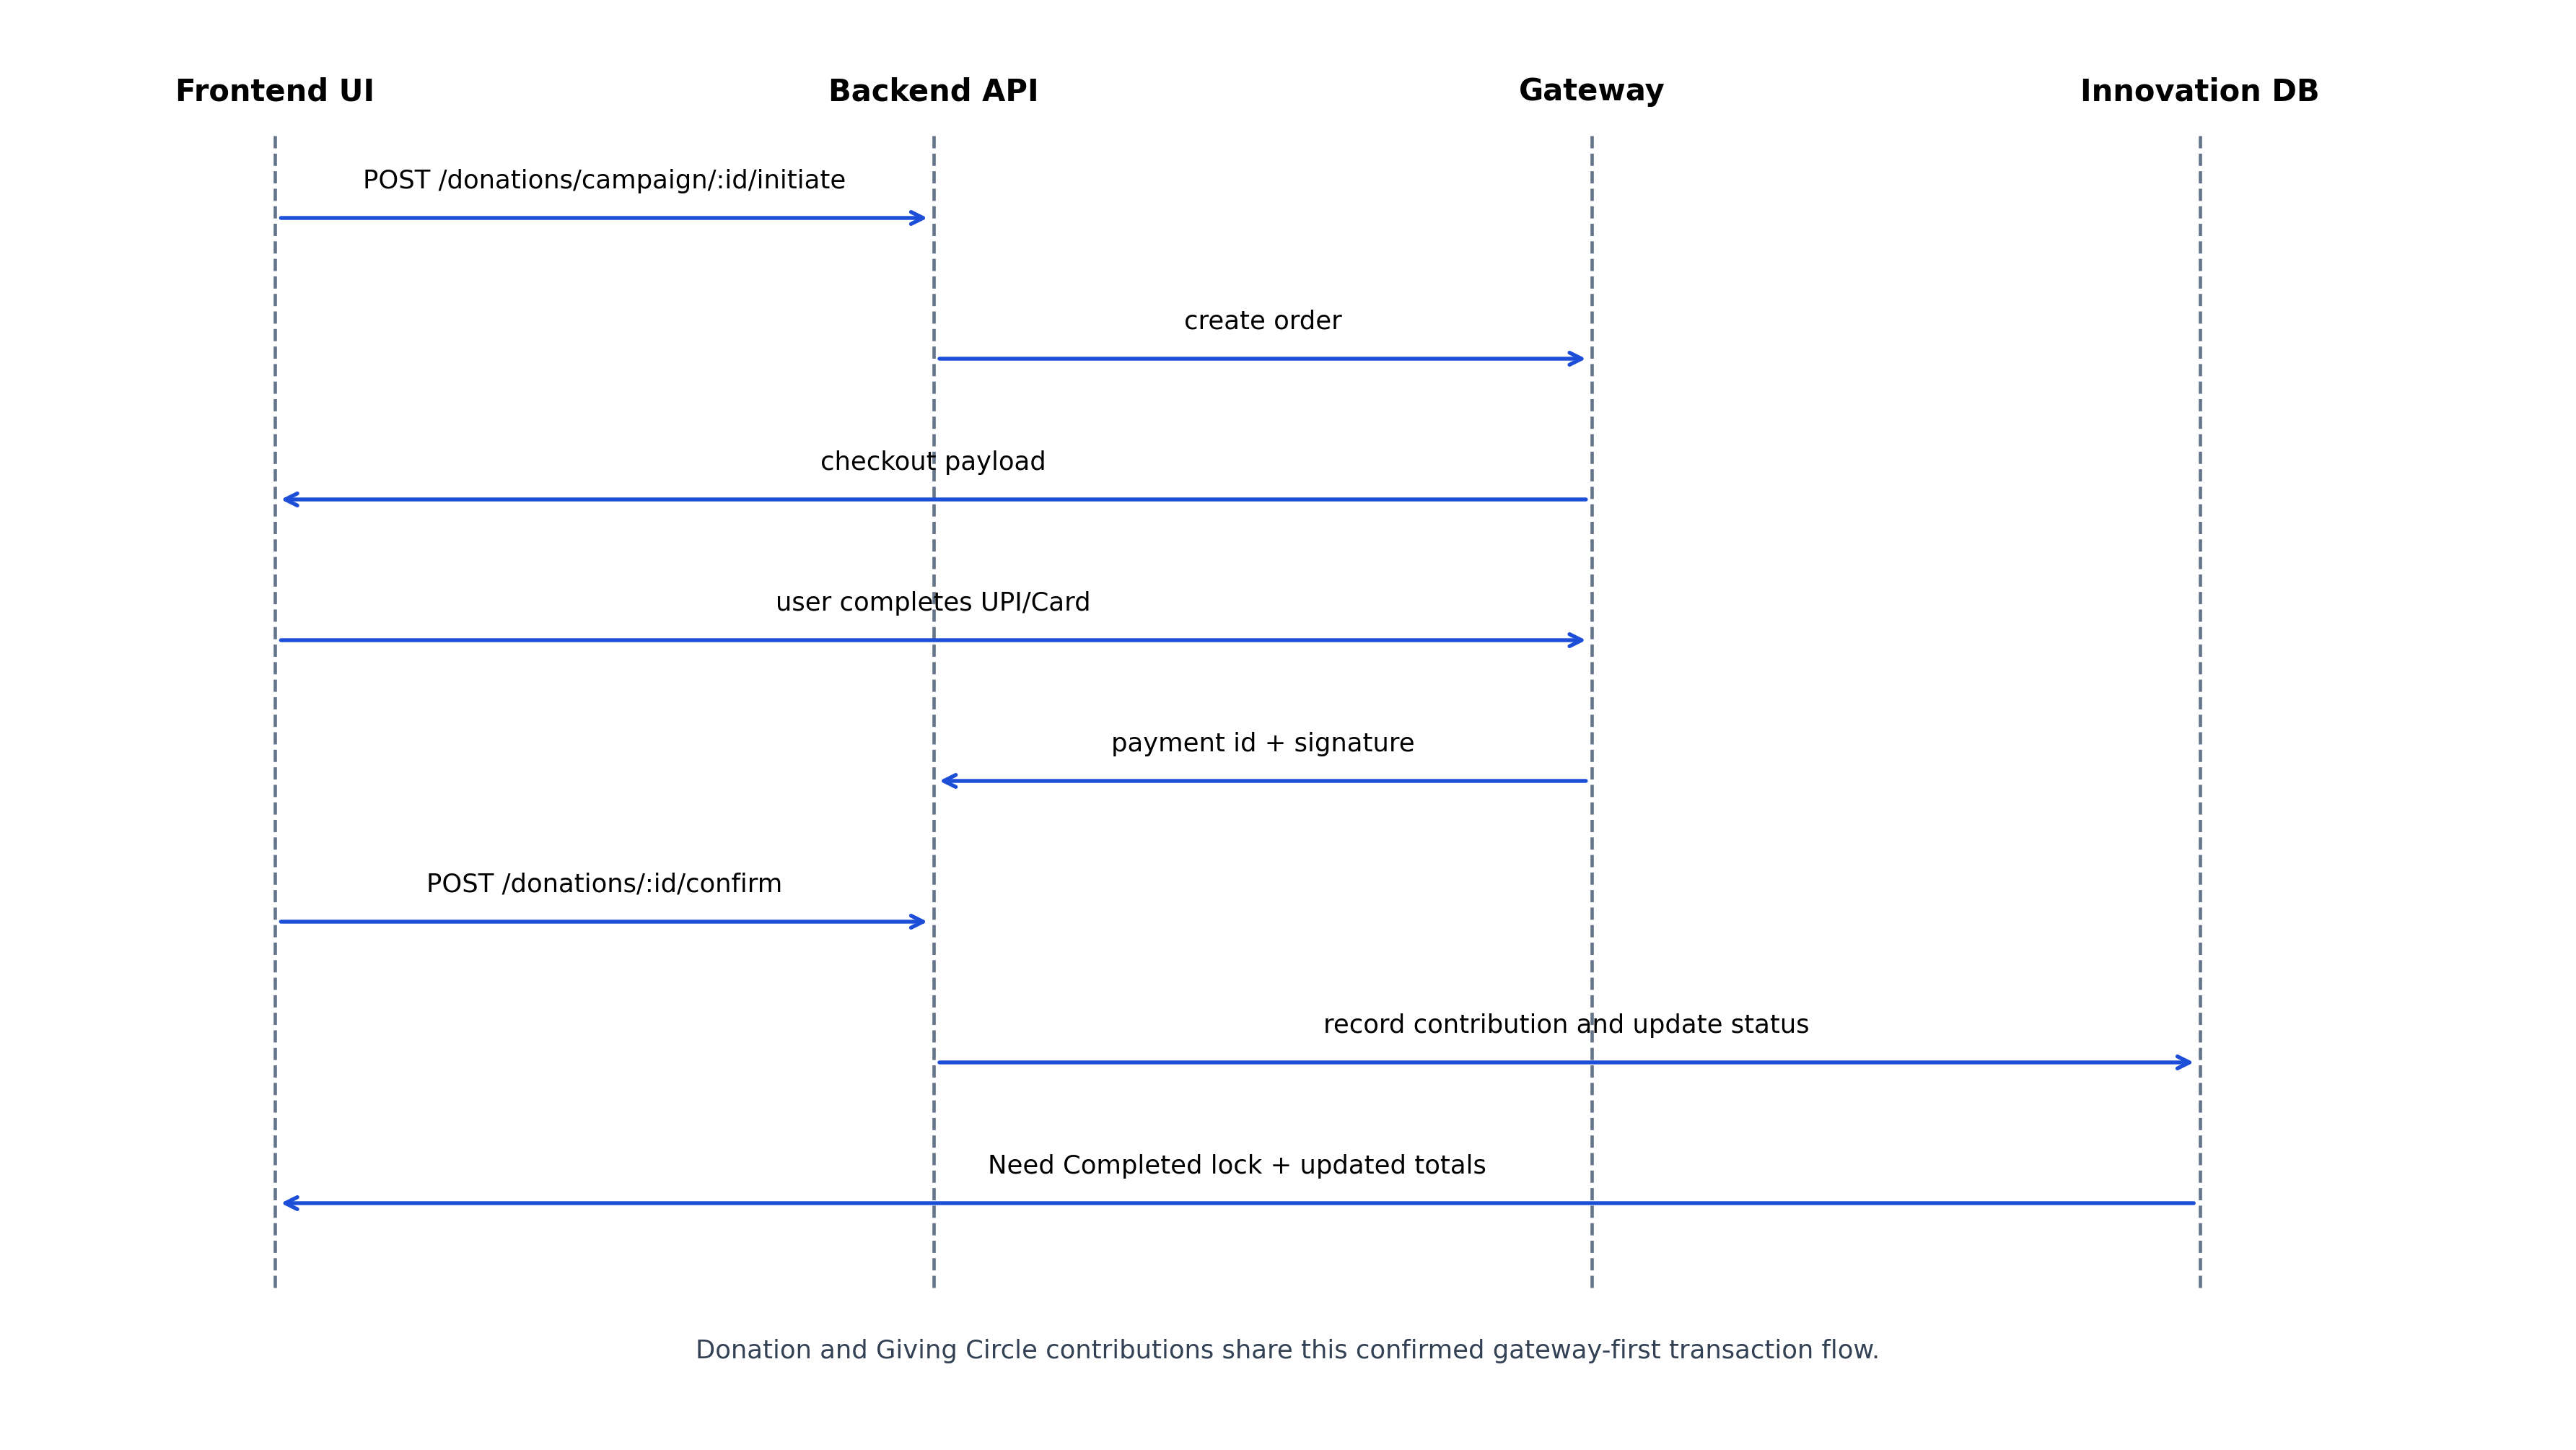
\includegraphics[width=\linewidth]{figures/payment_sequence.png}}
\caption{Gateway-confirmed contribution sequence used by donation and giving-circle flows.}
\label{fig:paymentseq}
\end{figure}

\subsection{Webhook Reliability Workflow}
The project includes signed outbound webhook delivery, dead-letter capture, automatic replay worker, metrics/export endpoints, and retention cleanup APIs for operational hygiene.

\begin{figure}[htbp]
\centerline{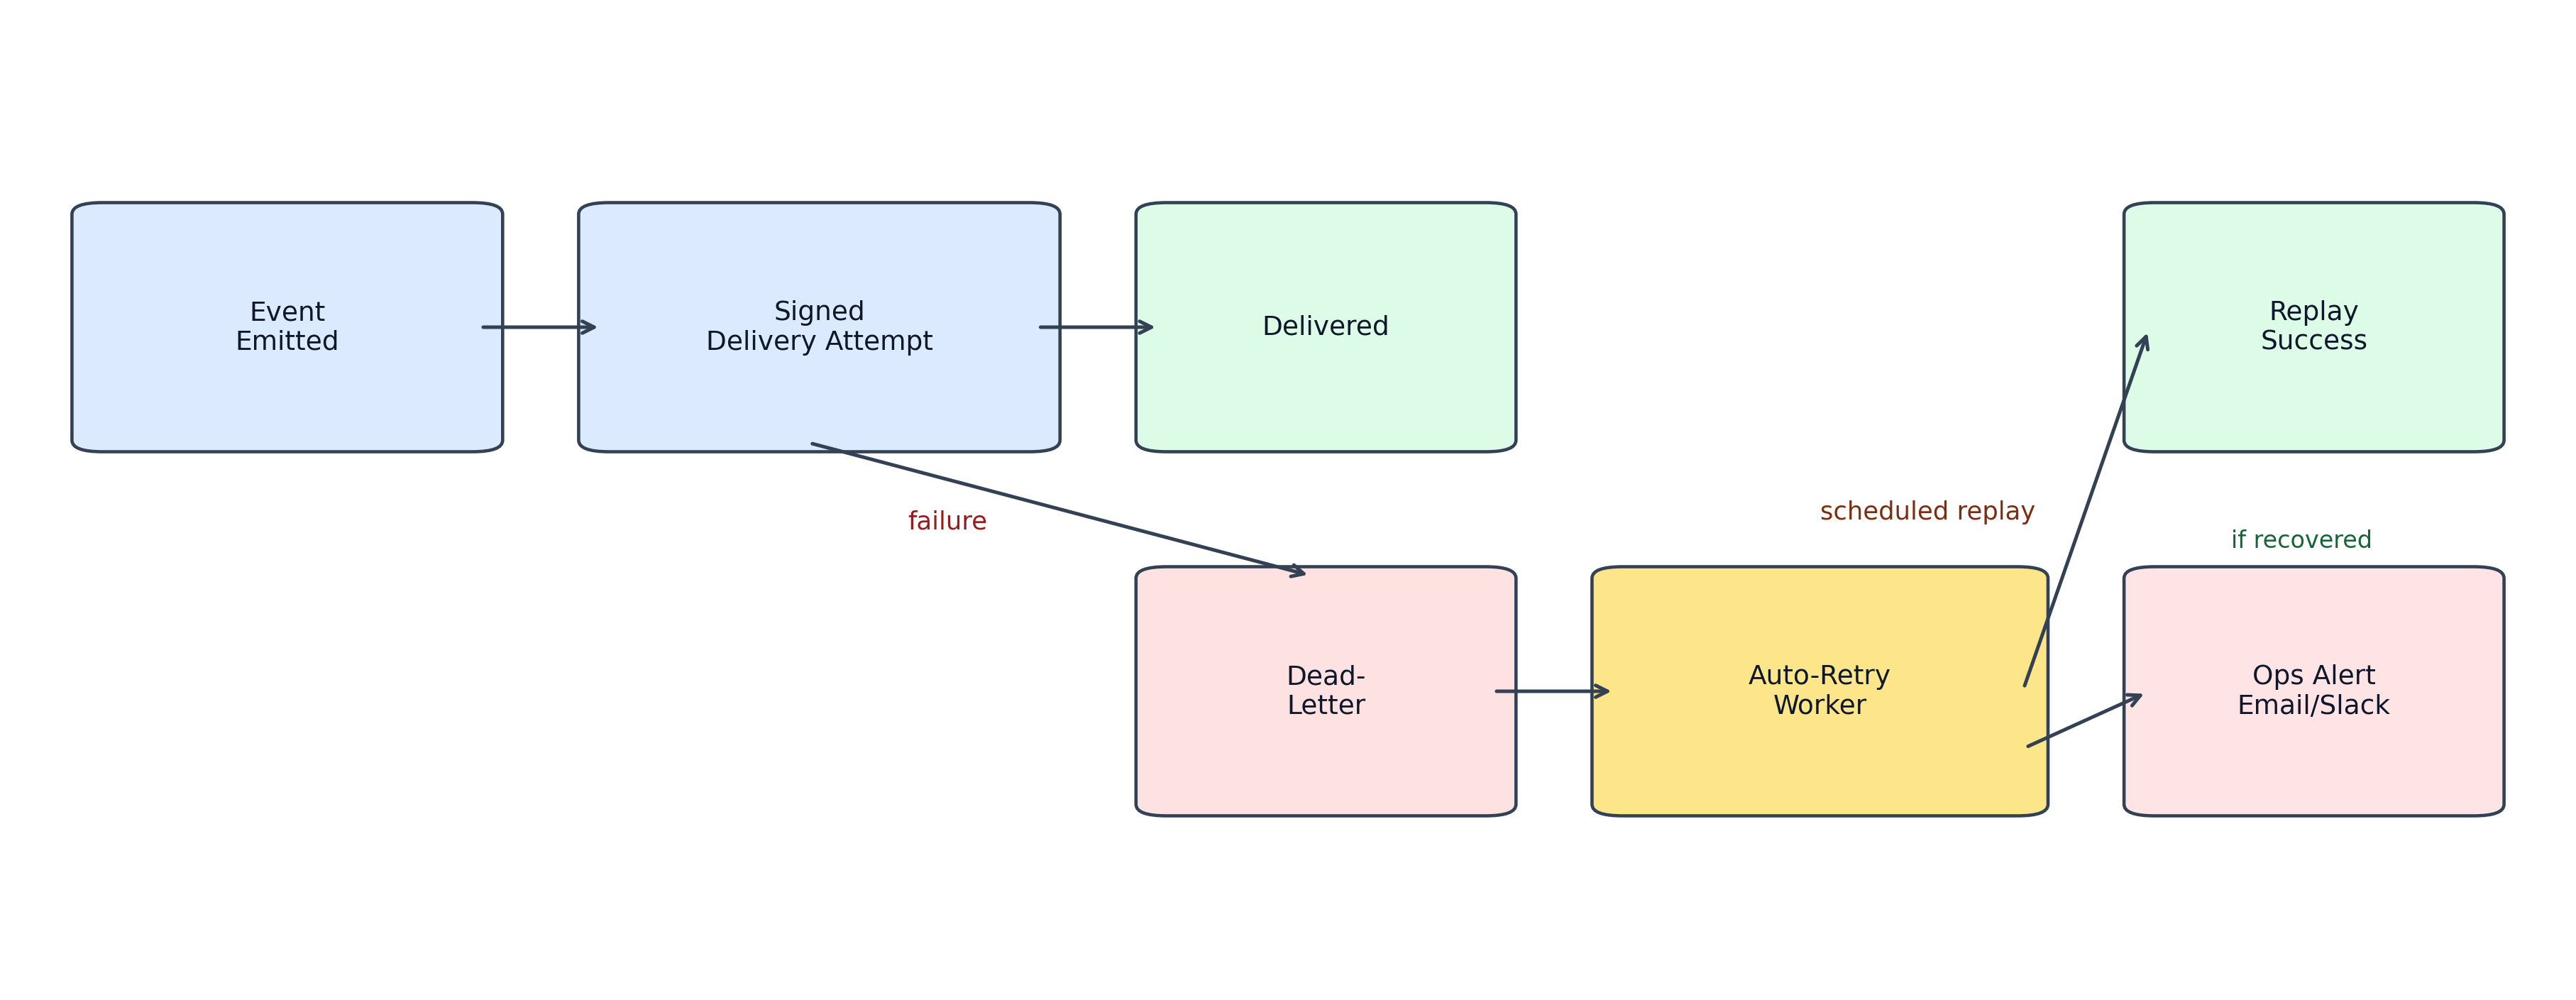
\includegraphics[width=\linewidth]{figures/webhook_lifecycle.png}}
\caption{Webhook delivery lifecycle with dead-letter replay and operations alerting.}
\label{fig:webhook}
\end{figure}

\section{Evaluation}
\subsection{Execution Setup}
Validation uses role-specific smoke tests across authentication, campaigns, donations, volunteering, certificates, innovation modules, support requests, messaging, moderation, and admin operations.

\subsection{Smoke-Test Latency Summary}
\begin{table}[htbp]
\caption{Smoke Execution Summary}
\begin{center}
\begin{tabular}{|l|c|}
\hline
\textbf{Metric} & \textbf{Observed Value} \\
\hline
Validated scenario steps & 35 \\
\hline
Average step latency & 21.69 ms \\
\hline
P90 step latency & 72 ms \\
\hline
Max observed step latency & 125 ms \\
\hline
\end{tabular}
\label{tab:smoke}
\end{center}
\end{table}

\begin{figure}[htbp]
\centerline{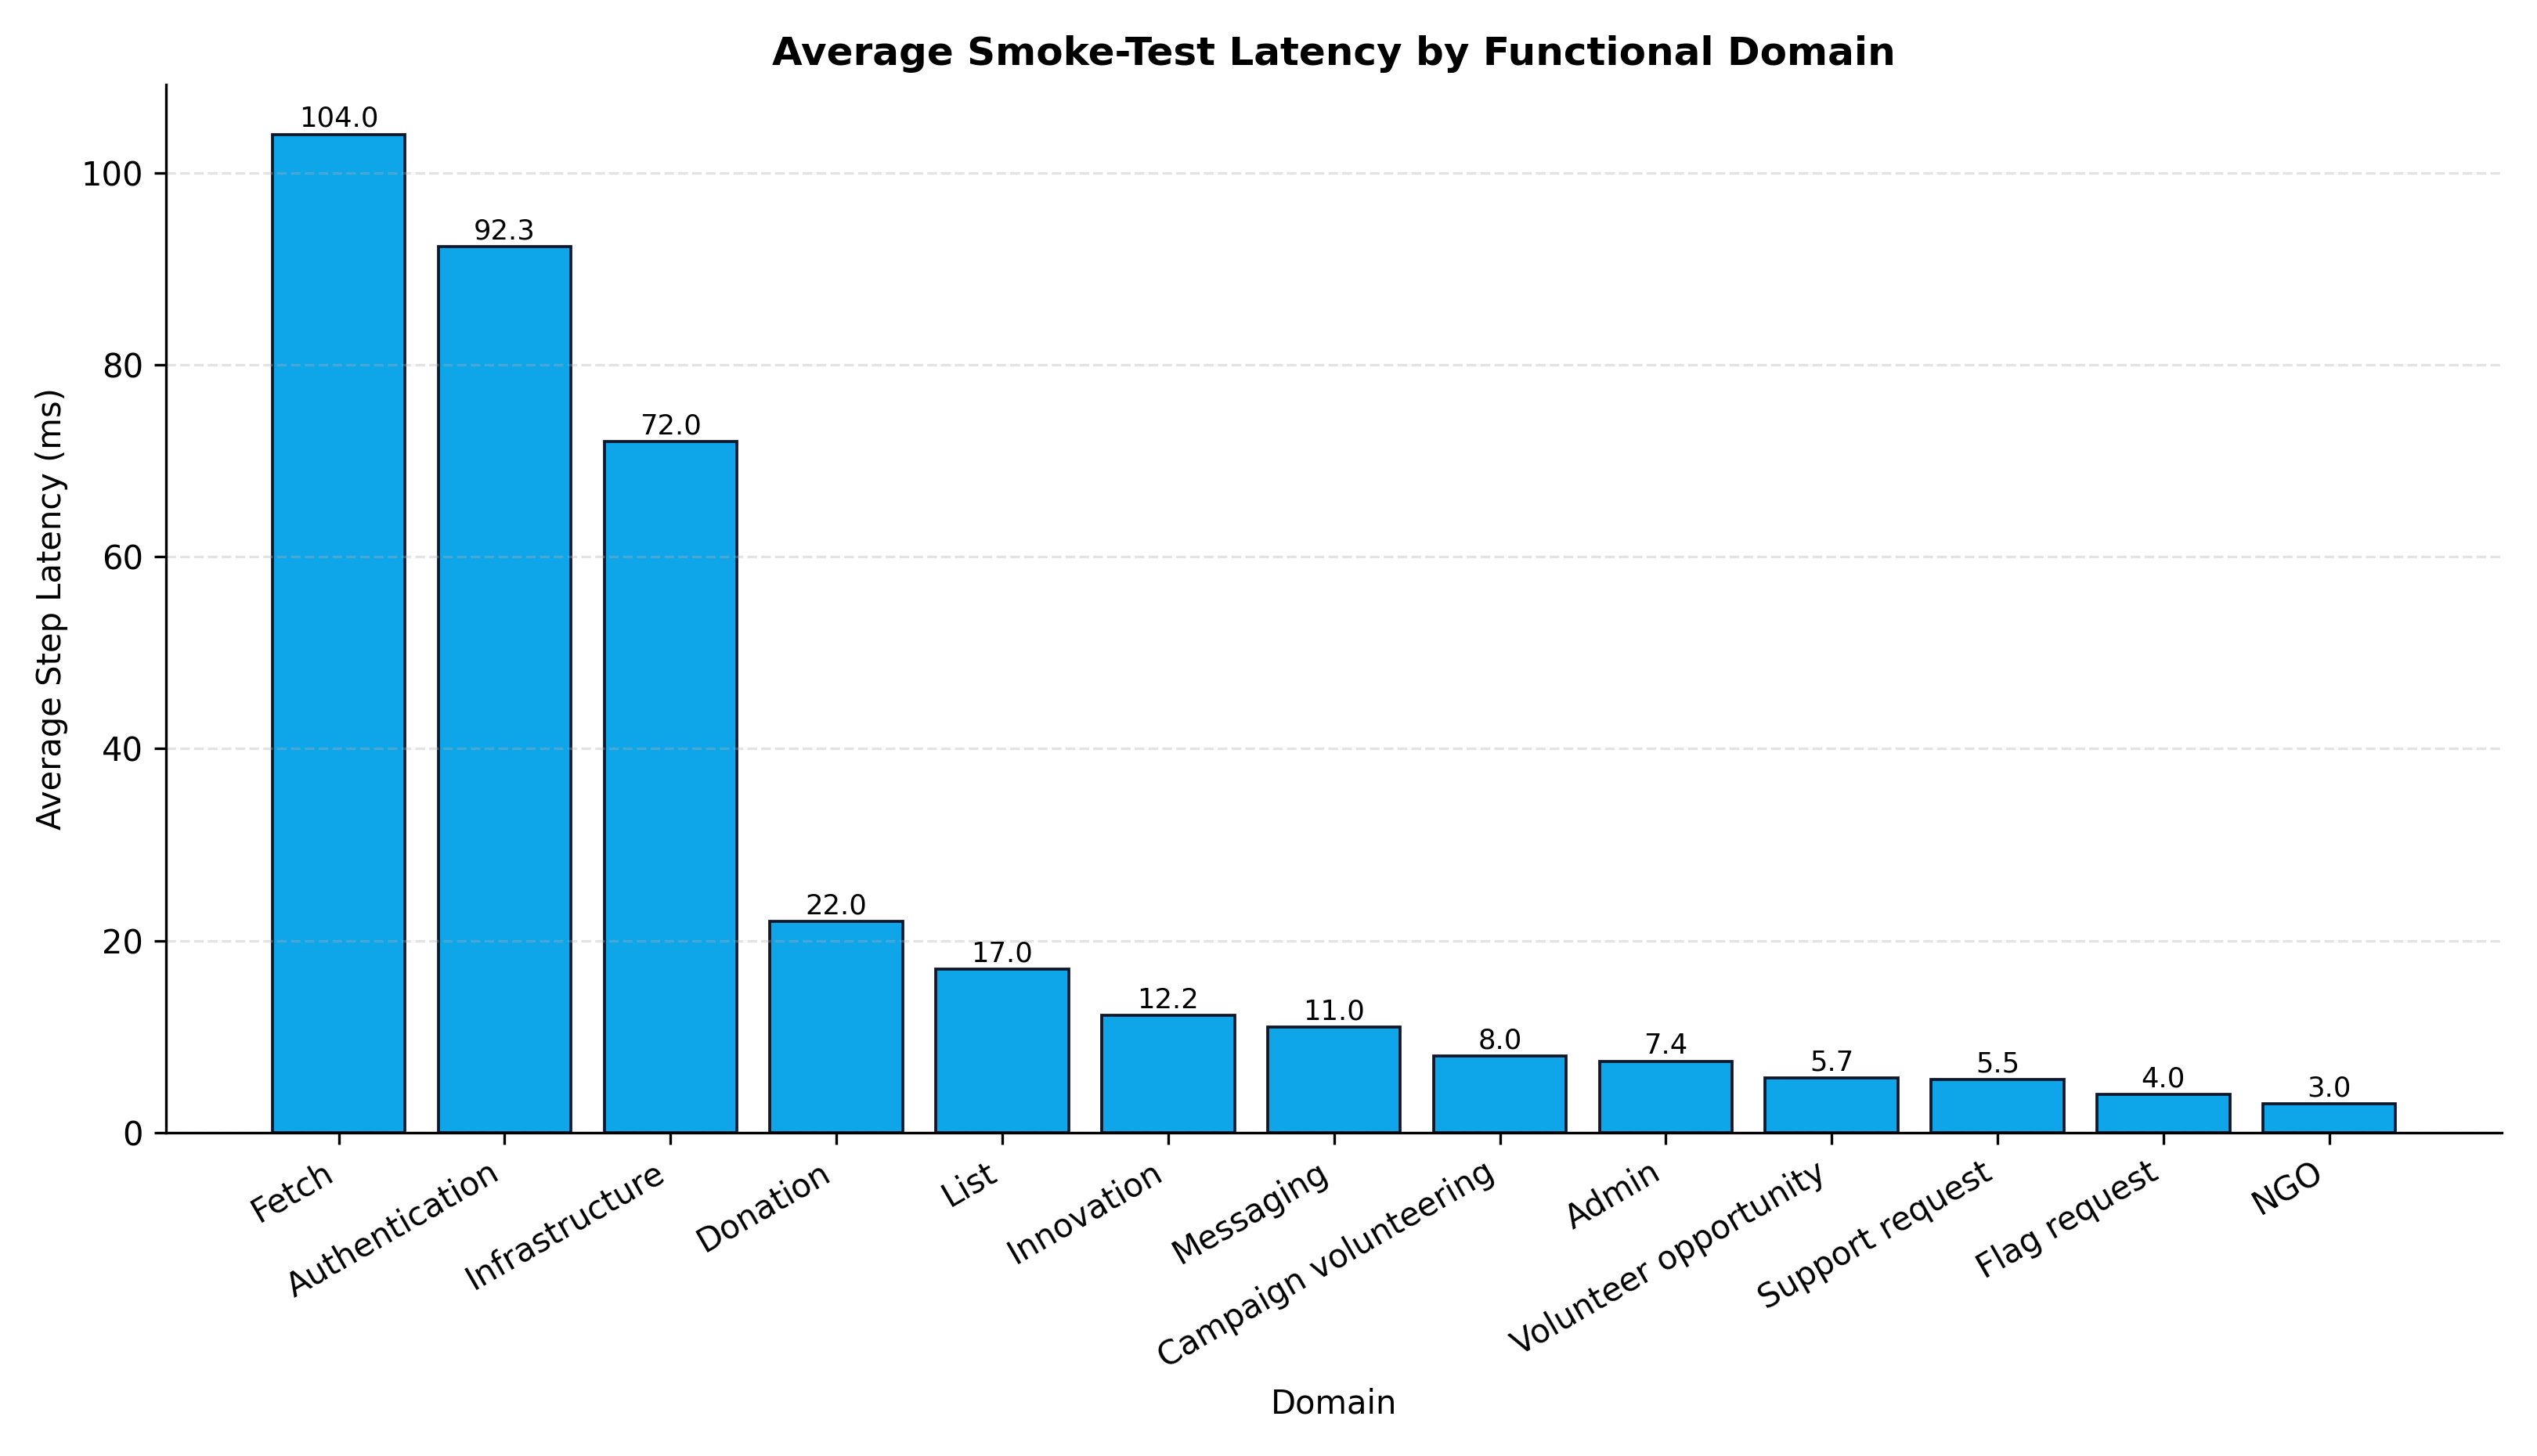
\includegraphics[width=\linewidth]{figures/smoke_latency_breakdown.png}}
\caption{Average latency by functional domain from smoke execution trace.}
\label{fig:smokebreakdown}
\end{figure}

\begin{table}[htbp]
\caption{Top Slowest Smoke Steps}
\begin{center}
\begin{tabular}{|p{5.8cm}|c|}
\hline
\textbf{Step} & \textbf{Latency (ms)} \\
\hline
Login as user & 125 \\
Fetch NGO profile & 104 \\
Login as NGO & 80 \\
API health & 72 \\
Login as admin & 72 \\
Admin dashboard snapshot & 40 \\
List NGOs & 27 \\
Innovation: CRM donors + segments & 26 \\
\hline
\end{tabular}
\label{tab:slowsteps}
\end{center}
\end{table}

\begin{figure}[htbp]
\centerline{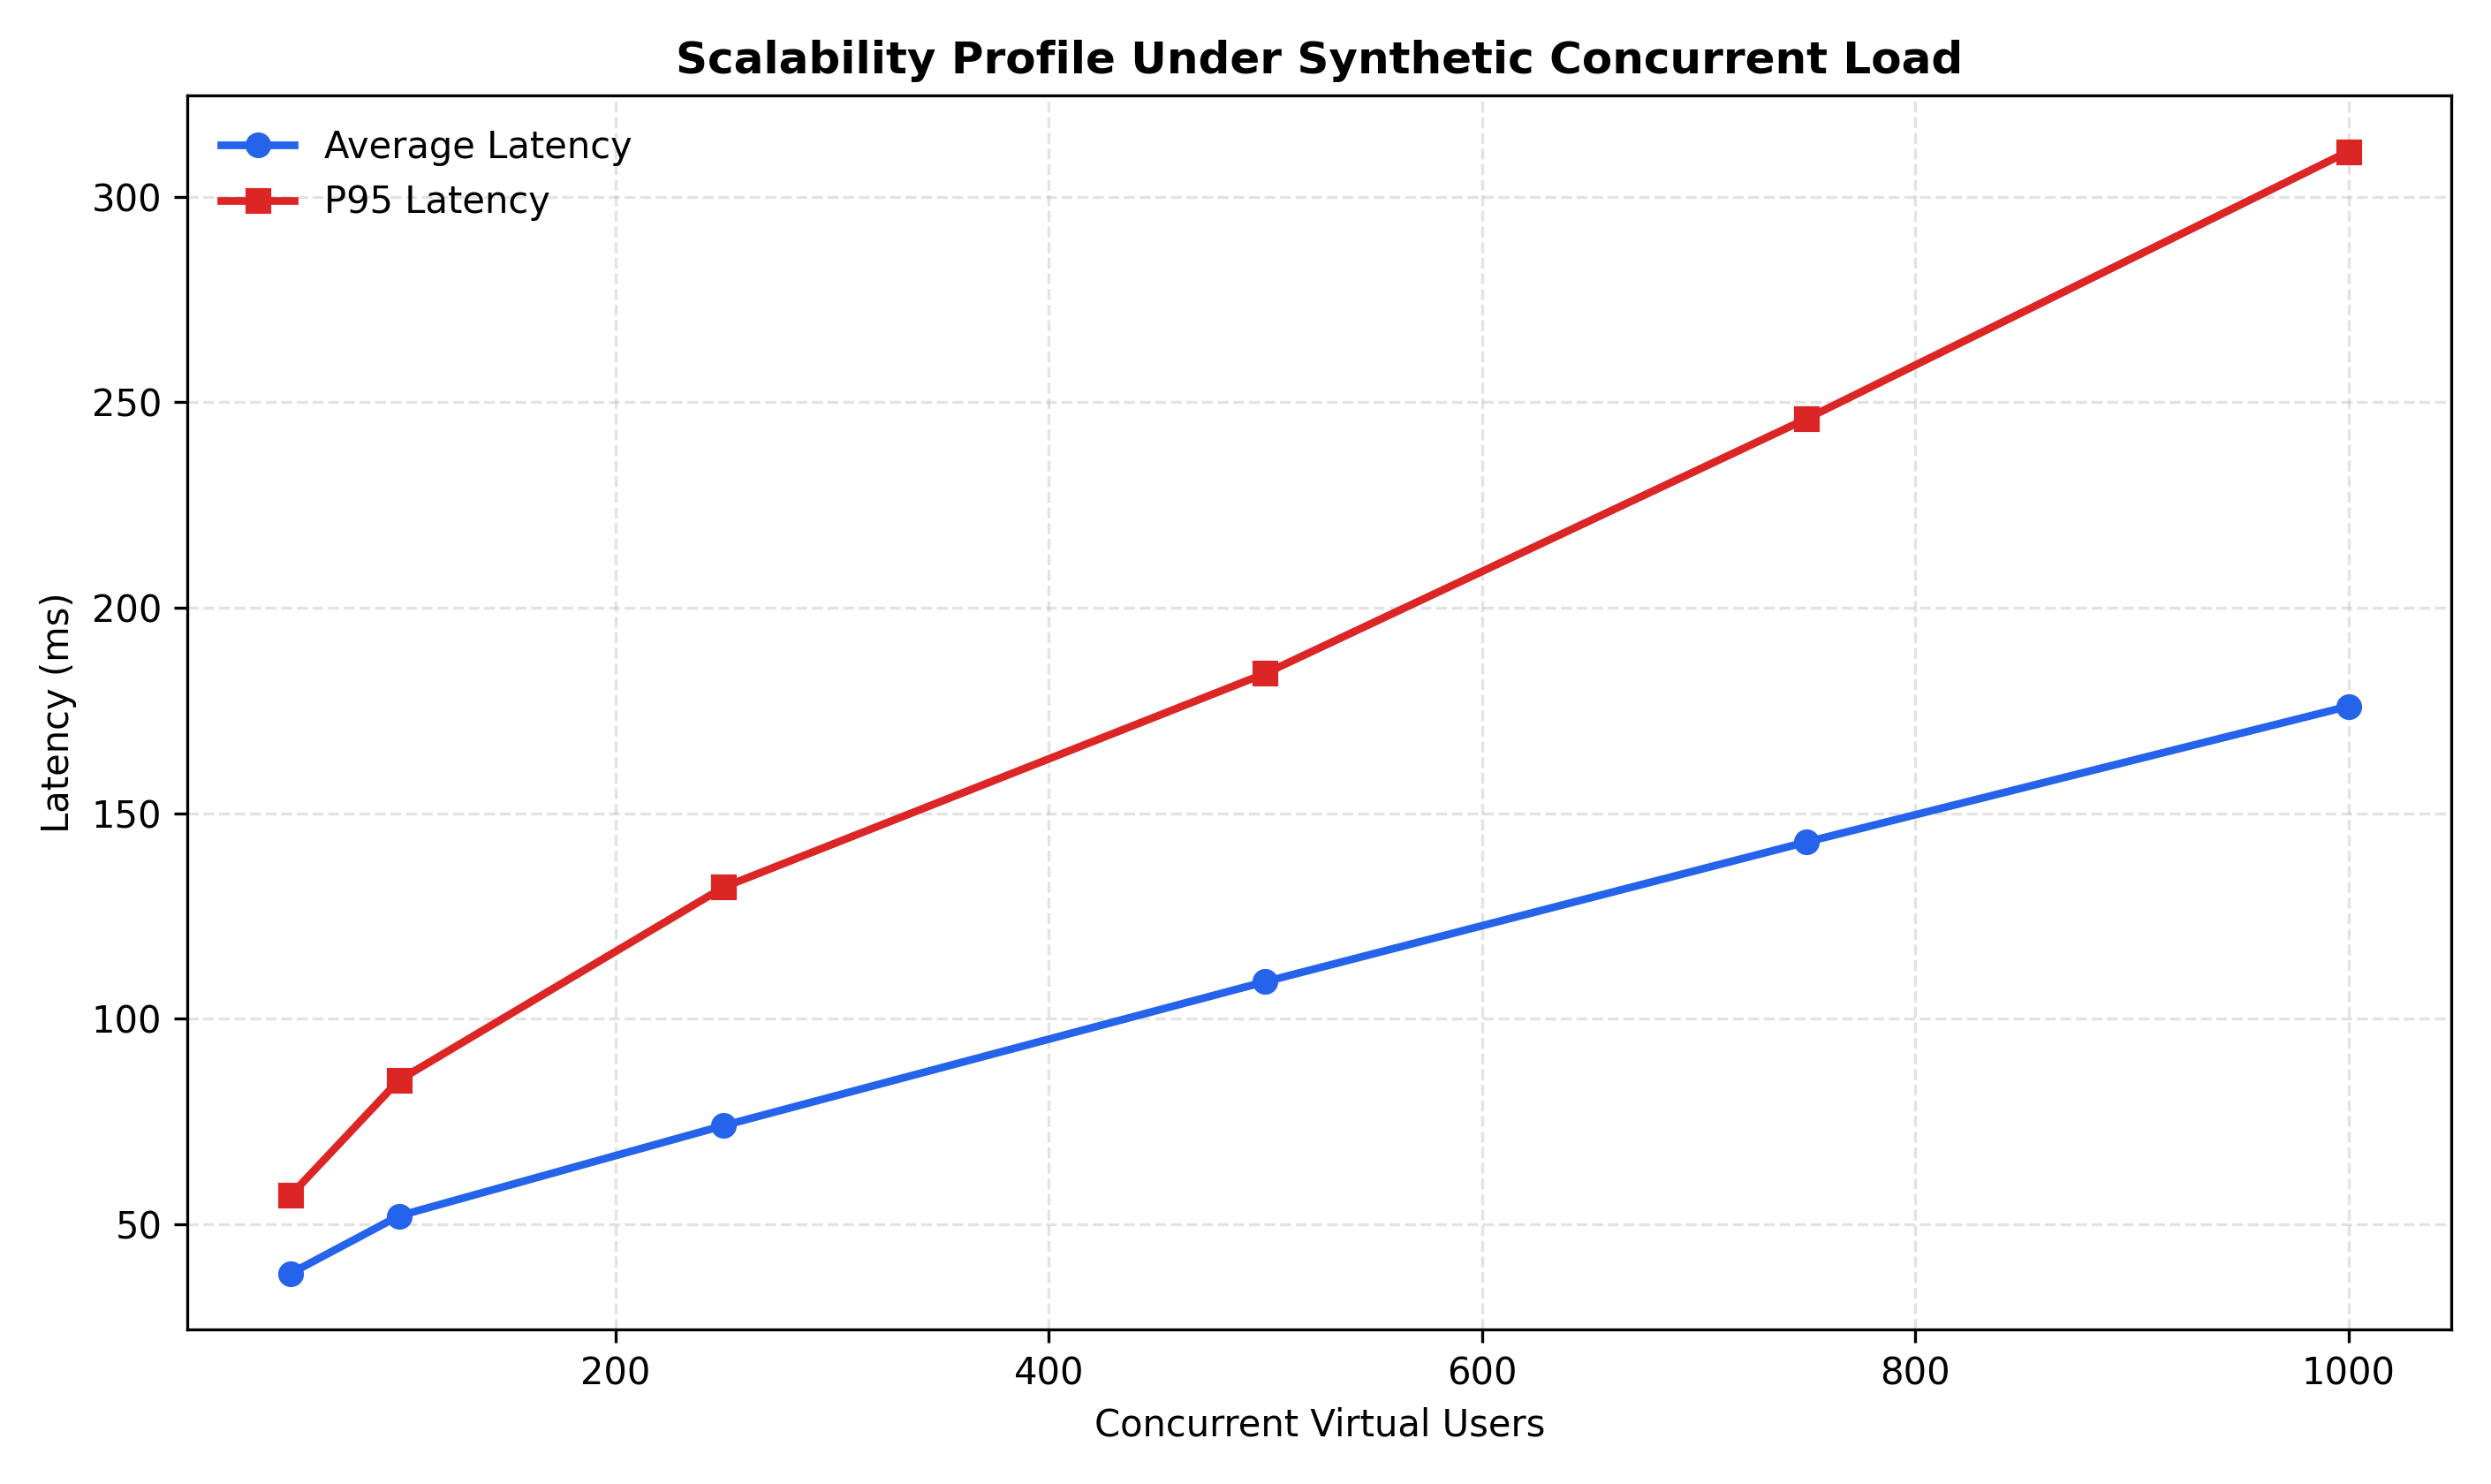
\includegraphics[width=\linewidth]{figures/scalability_latency.png}}
\caption{Synthetic scalability profile (average and p95 latency).}
\label{fig:scalability}
\end{figure}

\section{Discussion}
The updated platform demonstrates that broad feature coverage can coexist with low validation latency when modules are kept explicit and route ownership is clear. The largest endpoint concentrations are innovation and admin, which is expected due to operational breadth. JSONB plus typed relational columns provided schema flexibility without sacrificing joinability for analytics and moderation workflows.

Limitations remain. Smoke tests validate behavior breadth but are not a replacement for sustained soak testing. AI assistance quality also depends on prompt governance and source grounding, and payment/webhook production readiness depends on provider credentials, secret rotation, and monitoring discipline.

\section{Conclusion}
This work presents a complete, IEEE-style implementation report of NGO-Connect as an end-to-end digital philanthropy platform. The updated system integrates trust controls, innovation workflows, and operations reliability while maintaining practical performance in end-to-end validation. The architecture is suitable for extension into mobile offline clients, deeper analytics pipelines, and more advanced recommendation/risk models.

\section*{Acknowledgment}
The authors thank the Department of Computer Science and Engineering, CMR University, Bengaluru, for academic support and infrastructure.

\begin{thebibliography}{00}
\bibitem{reactdocs} Meta Open Source, ``React Documentation,'' 2026. [Online]. Available online: react.dev
\bibitem{expressdocs} OpenJS Foundation, ``Express 4.x API Reference,'' 2026. [Online]. Available online: expressjs.com
\bibitem{postgresdocs} PostgreSQL Global Development Group, ``PostgreSQL Documentation: JSON Types,'' 2026. [Online]. Available online: postgresql.org/docs
\bibitem{jwt} M. Jones, J. Bradley, and N. Sakimura, ``JSON Web Token (JWT),'' IETF RFC 7519, 2015.
\bibitem{rfc_tail} J. Dean and L. A. Barroso, ``The Tail at Scale,'' \textit{Communications of the ACM}, vol. 56, no. 2, pp. 74--80, 2013.
\bibitem{rag} P. Lewis \textit{et al.}, ``Retrieval-Augmented Generation for Knowledge-Intensive NLP Tasks,'' in \textit{NeurIPS}, 2020.
\bibitem{owaspapi} OWASP Foundation, ``OWASP API Security Top 10 -- 2023,'' 2023. [Online]. Available online: owasp.org/API-Security
\bibitem{gemini} Google for Developers, ``Gemini API Documentation,'' 2026. [Online]. Available online: ai.google.dev
\bibitem{razorpay} Razorpay, ``Razorpay API Reference,'' 2026. [Online]. Available online: razorpay.com/docs/api
\bibitem{nist} NIST, ``Digital Identity Guidelines (SP 800-63B),'' 2020.
\bibitem{jaccard} P. Jaccard, ``Etude comparative de la distribution florale,'' \textit{Bull. Soc. Vaudoise Sci. Nat.}, vol. 37, pp. 547--579, 1901.
\bibitem{ndcg} K. Jarvelin and J. Kekalainen, ``Cumulated gain-based evaluation of IR techniques,'' \textit{ACM TOIS}, vol. 20, no. 4, pp. 422--446, 2002.
\end{thebibliography}

\end{document}
